\subsubsection{{Similaridade}}

De forma concisa, similaridade consiste em realizar uma buscar dentro de uma imagem específica com o objetivo de reconhecer/encontrar objetos semelhantes a um modelo de busca. Nessas funções de busca por similaridade são utilizados cálculos de vetores de características para realizar as comparações de igualdade \cite{MAIZA2013}.

Os seres humanos possuem uma grande facilidade de reconhecer informações apresentadas de maneira visual, onde consequentemente são capazes, com grande facilidade, de interpretar imagens diversificadas sem grande esforço. Exemplificando esta situação, os seres humanos consegue distinguir de forma fácil a diferença entre um círculo grande e um círculo pequeno, um quadrado grande de um quadrado pequeno, a diferença entre um triângulo e um quadrado de tamanhos idênticos, dentre outros. Conforme \citeonline{SILVA2009} relata em seu artigo, com a tecnologia disponível atualmente para realizar a construção de aplicações capazes de identificar informações dentro de uma imagem ainda é muito ineficiente, quando comparada com a capacidade humana.

Segundo \citeonline{MAIA2013}, algoritmos de similaridade trabalham com métricas que informam o quanto uma imagem é parecida com a outra. Ou seja, pode-se aplicar essas métricas utilizando padrões de buscas a fim de uma análise mais específica. De forma estatística, \citeonline{MAIA2013} completam que possui dois tipos básicos de medidas de similaridade: correlação e coseno. Seguindo o contexto do artigo, a similaridade por correlação entre dois vetores retorna um valor booleano, ou seja, 0 e 1, onde o valor de retorno igual a 1 significa que há uma similaridade forte naquele ponto, ou seja, os valores dos vetores são parecidos e, se o retorno for 0, não existe correlação. No entanto, o autor enfatiza a presença de um retorno igual a -1, no qual a similaridade daquele ponto é inversa ao padrão de busca. Ja a similaridade por coseno é similar a correlação, no qual o retorno também e 0 e 1, porém nesse método é analisado o tamanho do vetor e a formação de um ângulo entre os mesmos. Quanto mais próximo de 1 for o valor, mais similares são os vetores.

% Comentário de múltiplas linhas
\begin{comment}
Agregando o assunto supracitado, \citeonline{MAIZA2013}, \citeonline{MAIA2013} utilizam em seus artigos a função euclidiana para realizar cálculos de distâncias nas estruturas. Essa função utiliza métricas de similaridade para calcular a distância entre dois vetores de características, percorrendo o vetor apenas uma vez. A distância euclidiana entre dois pontos (Xi e Xj) é definida através da equação:
\end{comment}

\citeonline{MAIZA2013}, \citeonline{MAIA2013} utilizam em seus artigos a função euclidiana para realizar cálculos de distâncias nas estruturas. Essa função utiliza métricas de similaridade para calcular a distância entre dois vetores de características, percorrendo o vetor apenas uma vez. A distância euclidiana entre dois pontos (Xi e Xj) é definida através de uma equação matemática, na qual não faz parte do escopo deste projeto.

\begin{comment}

%\begin{flalign*}
   d = \sqrt{\sum_{k=1}^{n} (X_{ik} - X_{jk})^2} \\
\end{flalign*}

onde:

\begin{math} X_{ik} \end{math} e \begin{math} X_{jk} \end{math} para k = 1, e \textbf{n} as quantidades de atributos presentes nas instâncias \begin{math} X_{ik} \end{math}, \begin{math} X_{jk} \end{math}. \newline

Segundo \citeonline{MAIA2013}, a distância euclidiana necessita que quatro condições, nos vetores a, b e c, sejam validas para atuar como medida:

%\begin{enumerate}
%    \item d(a, b) \begin{math} \ge \end{math} 0;
%    \item d(a, a) = 0;
%    \item d(a, b) = d(b, a);
%    \item d(a, c) \begin{math} \le \end{math} d(a, b) + d(b, c).
%\end{enumerate}

\begin{enumerate}
    \item A distância do vetorA até o vetorB tem que ser maior ou igual a 0;
    \item A distância do vetorA até o vetorA tem que ser igual a 0, ou seja, os vetores tem que ser iguais;
    \item A distância do vetorA até o vetorB tem que ser igual a distância do vetorB até o vetorA;
    \item A distância do vetorA até o vetorC tem que ser menor ou igual a distância do vetorA até o vetorB mais a distância do vetorB até o vetorC.
\end{enumerate}

Segundo \citeonline{MAIA2013}, a distância euclidiana necessita que quatro condições nos vetores de comparação A, B e C, sejam validas para atuar como medida:

\begin{enumerate}
    \item A distância do vetorA até o vetorB tem que ser maior ou igual a 0;
    \item A distância do vetorA até o vetorA tem que ser igual a 0, ou seja, os vetores tem que ser iguais;
    \item A distância do vetorA até o vetorB tem que ser igual a distância do vetorB até o vetorA;
    \item A distância do vetorA até o vetorC tem que ser menor ou igual a distância do vetorA até o vetorB mais a distância do vetorB até o vetorC.
\end{enumerate}

O autor completa que o tamanho dos vetores influencia diretamente no desempenho da função de similaridade por distância, ou euclidiana.

\clearpage

\begin{figure}[!h]
\caption{{\footnotesize Exemplo do uso da distância Euclidiana.}}
 
\centering % para centralizarmos a figura
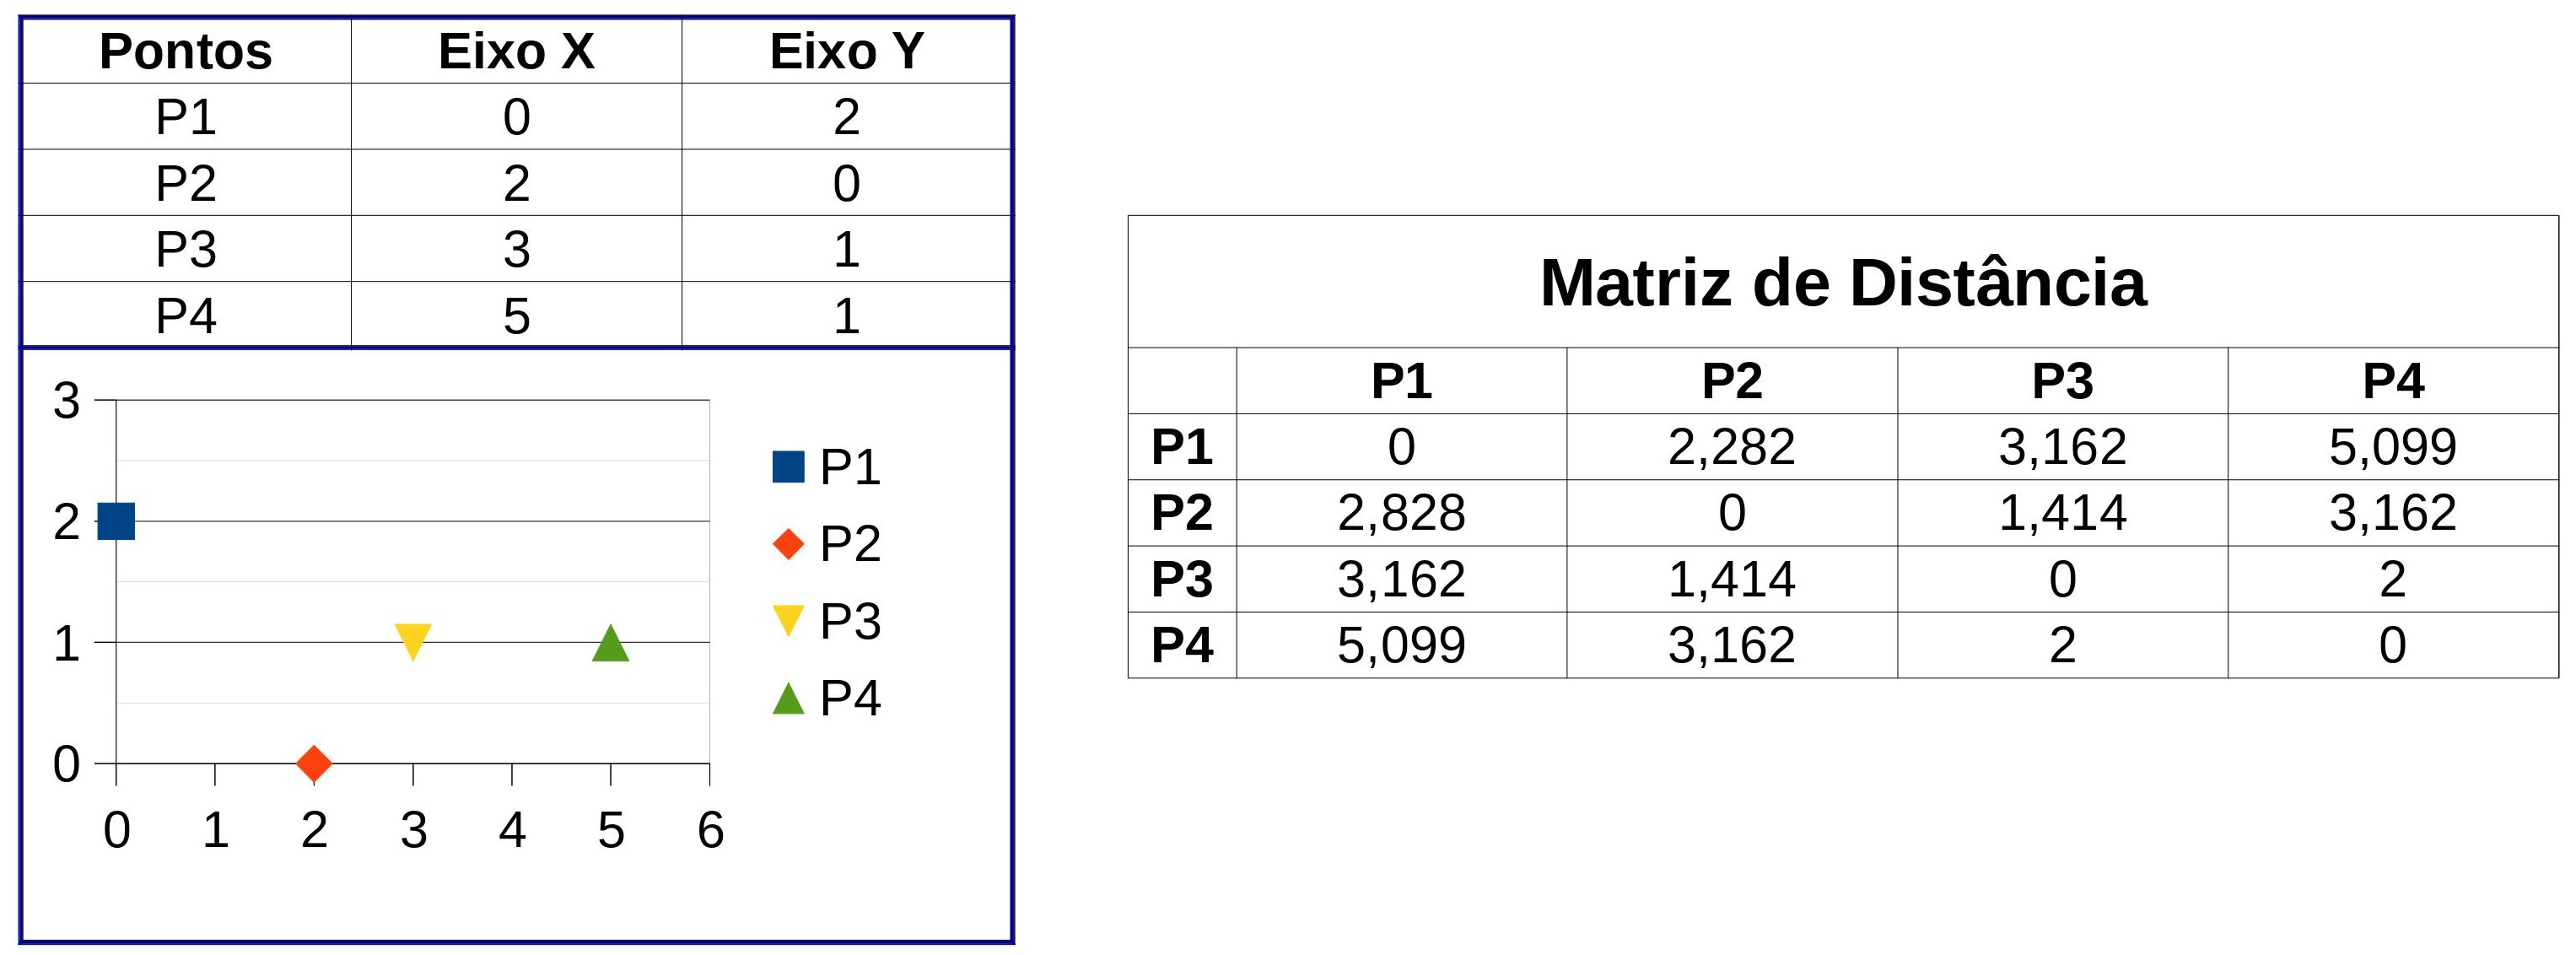
\includegraphics[width=10cm]{revisao-bibliografica/Figuras/Euclidiana.jpg}% leia abaixo
\label{figura:figura8}

\centering \subfloat {\footnotesize {Adaptado de: http://www.dsc.ufcg.edu.br/~pet/jornal/novembro2012/materias/recapitulando.html}}
{
\label{figura:figura8}
}
\end{figure}
%\clearpage
\end{comment}